\chapter{背景介绍}
\label{chap:background}

随着大规模预训练语言模型（Large Language Models, LLMs）在自然语言处理及更广泛的人工智能领域取得巨大成功，模型规模的持续扩张成为提升性能的关键驱动力。然而，由此带来的计算资源和训练成本的指数级增长，促使学术界和工业界探索更高效的模型架构。混合专家模型（Mixture-of-Experts, MoE）作为一种实现条件计算（conditional computation）的有效范式，能够在不显著增加计算量的前提下，将模型参数量扩展到数万亿级别，成为构建前沿大语言模型的核心技术之一。本章将介绍理解MoE模型所必需的背景知识，主要包括作为现代大语言模型基石的Transformer架构、混合专家模型的基本原理，以及预训练大语言模型的演进脉络。

\section{Transformer 架构回顾}

自Vaswani等人在2017年提出以来，Transformer架构凭借其核心的自注意力机制（Self-Attention Mechanism），彻底改变了序列到序列（sequence-to-sequence）任务的处理方式，并迅速成为自然语言处理领域的标准架构 \cite{Vaswani2017AttentionIA}。其并行处理能力和对长距离依赖的出色建模，为后续大规模预训练模型的诞生奠定了基础。

\paragraph{编码器-解码器结构}
原始的Transformer模型（图\ref{fig:trm}）包含一个编码器（Encoder）和一个解码器（Decoder）。编码器负责将输入序列（例如，一种语言的句子）映射为一系列连续的向量表示。解码器则基于这些向量表示，以自回归（auto-regressive）的方式逐个生成输出序列的标记。后续发展出的许多大规模语言模型，如BERT \cite{Devlin2019BERTPO}，采用了仅编码器（Encoder-only）的架构；而GPT系列模型 \cite{Radford2018ImprovingLU} 则采用了仅解码器（Decoder-only）的架构，后者在生成任务中尤为流行。

\begin{figure}[h]
    \centering
    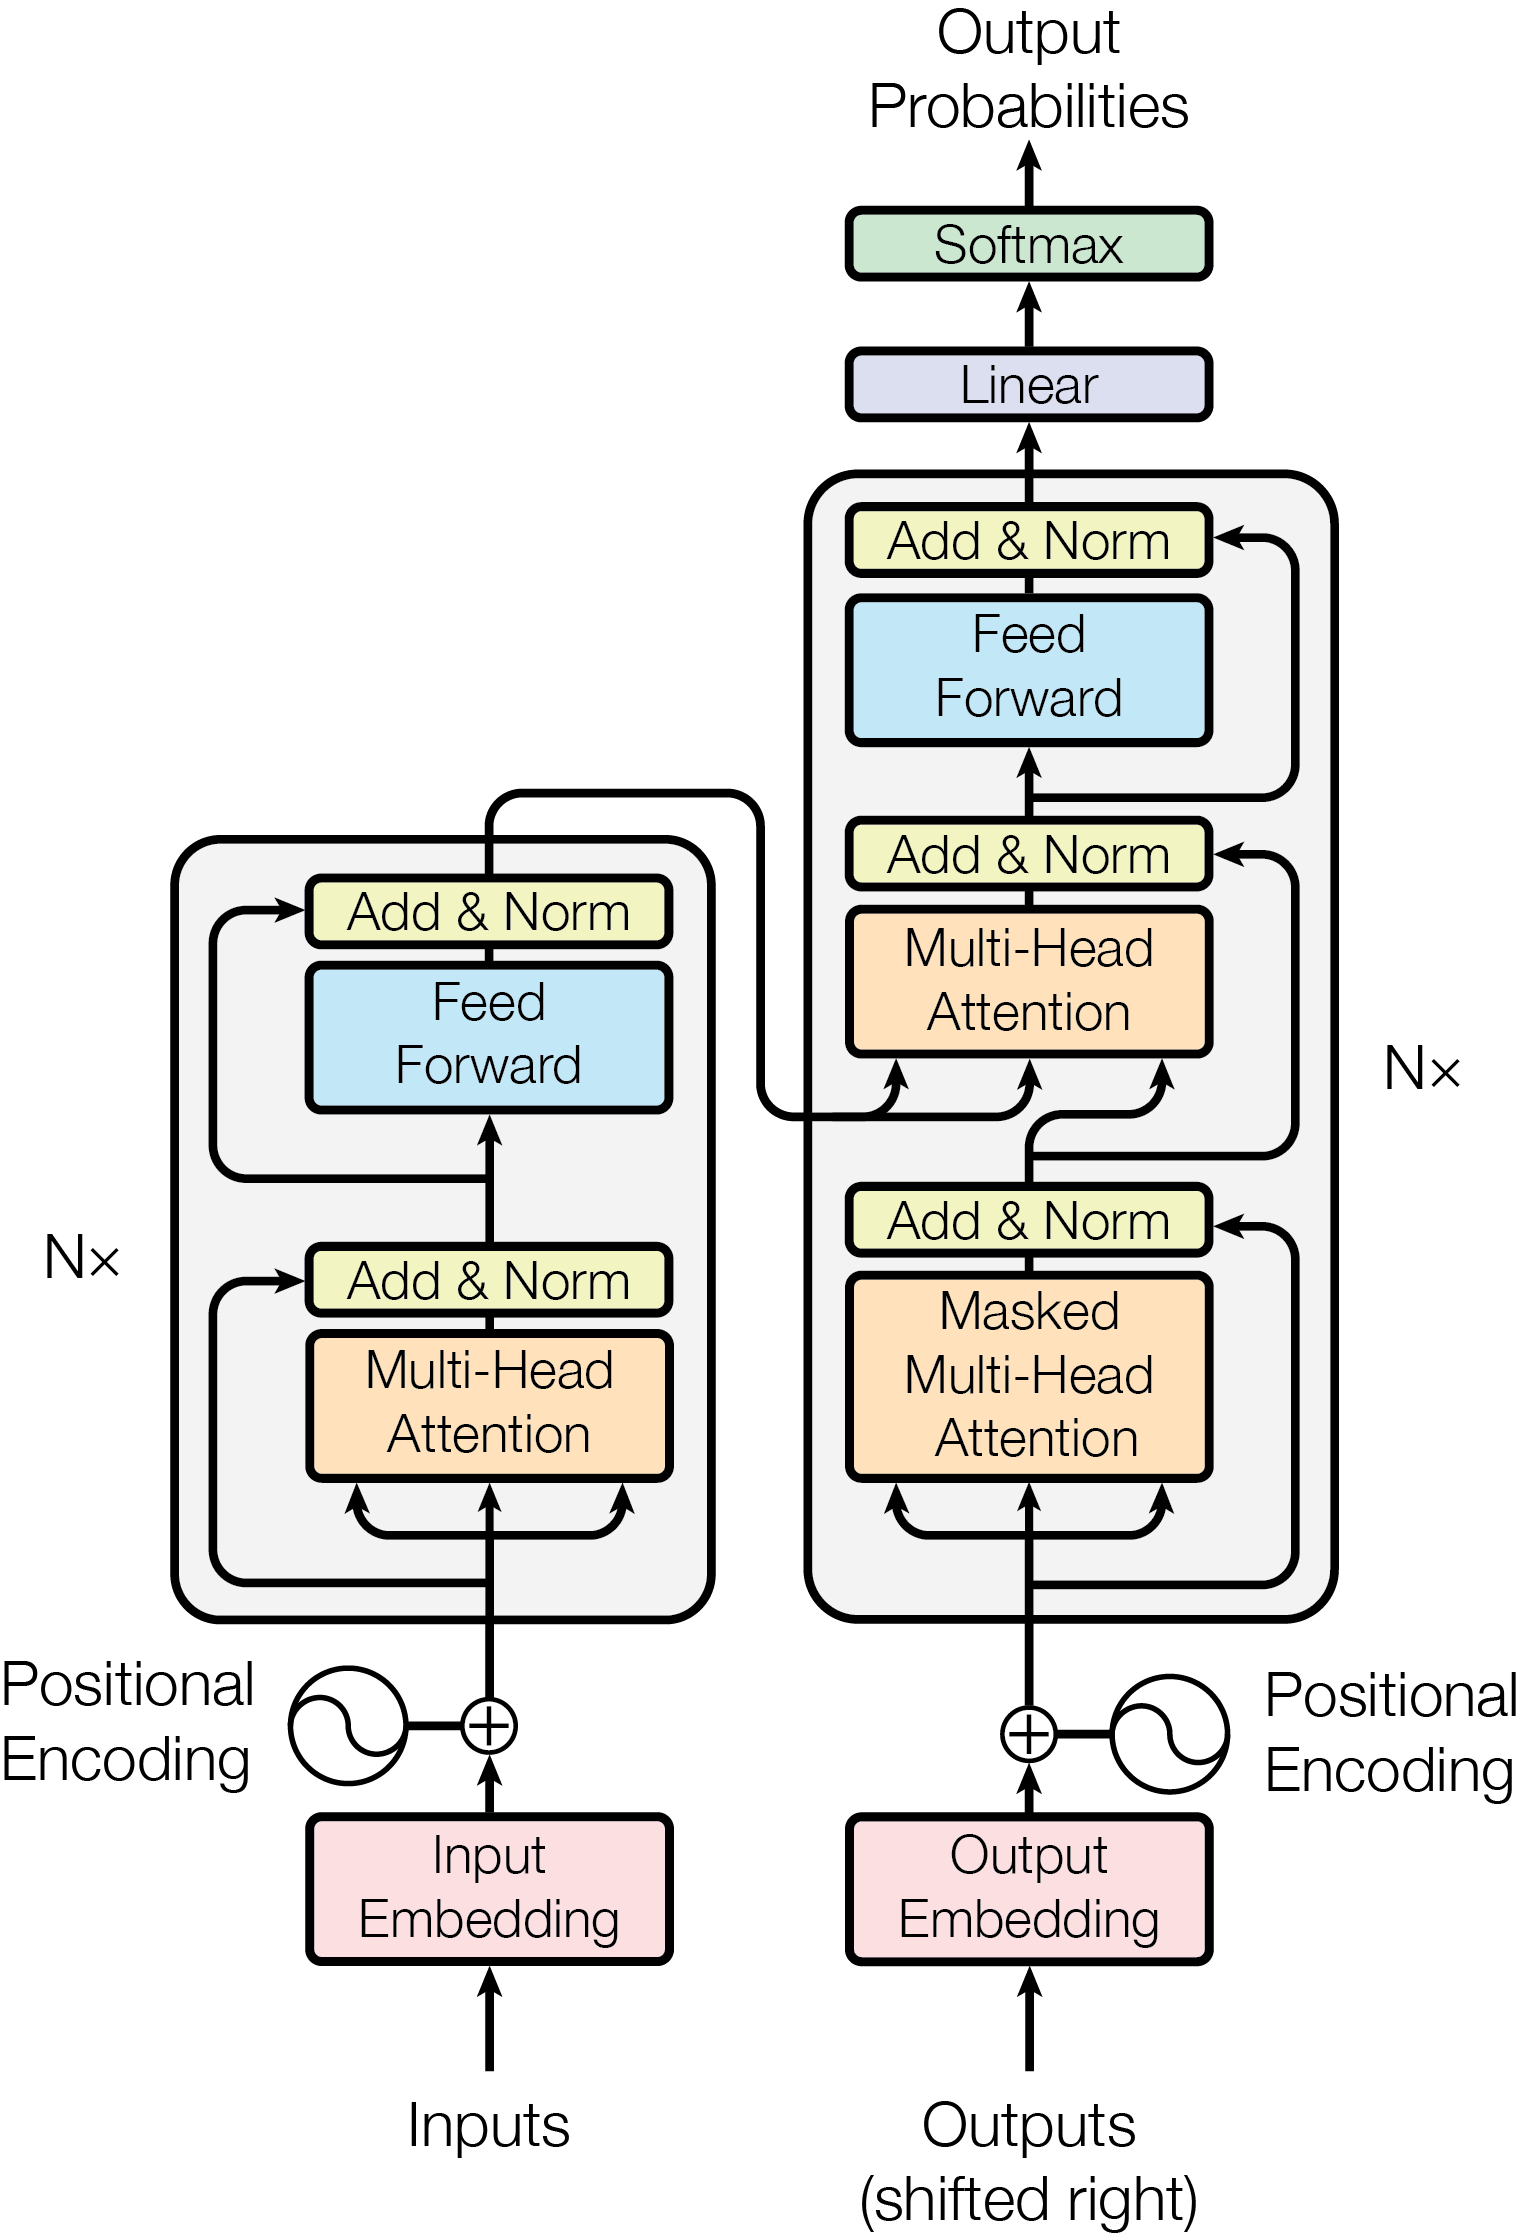
\includegraphics[width=0.6\linewidth]{figures/transformer.png}
    \caption{原始的Transformer模型架构\cite{Vaswani2017AttentionIA}，包含一个编码器和一个解码器。}
    \label{fig:trm}
\end{figure}

\paragraph{自注意力机制}
自注意力机制是Transformer的核心。它允许模型在处理一个序列时，为序列中的每个标记动态地计算其与序列中所有其他标记的关联权重。具体来说，对于每个输入标记，模型会生成三个向量：查询向量（Query, Q）、键向量（Key, K）和值向量（Value, V）。其核心计算过程为“缩放点积注意力”（Scaled Dot-Product Attention），其公式如下：
\begin{equation}
\text{Attention}(Q, K, V) = \text{softmax}\left(\frac{QK^T}{\sqrt{d_k}}\right)V.
\end{equation}
其中，$Q, K, V$ 分别代表由输入序列的查询、键、值向量堆叠而成的矩阵。$d_k$ 是键向量的维度。计算查询矩阵 $Q$ 和键矩阵转置 $K^T$ 的点积，得到原始的注意力得分。除以缩放因子 $\sqrt{d_k}$ 是为了防止点积结果过大，导致softmax函数进入梯度极小的区域，从而稳定训练过程。最后，归一化后的注意力权重会应用于值矩阵 $V$，得到加权的输出表示。

\paragraph{前馈网络}
Transformer的每个编码器和解码器层中，除了注意力子层外，还包含一个位置全连接的前馈网络（Position-wise Feed-Forward Network, FFN）。该网络通常由两个线性变换和一个非线性激活函数组成。对于注意力子层的输出向量 $x$，其计算过程可以表示为：
\begin{equation}
\text{FFN}(x) = \sigma(xW_1 + b_1) W_2 + b_2.
\end{equation}
其中，$W_1, b_1$ 和 $W_2, b_2$ 分别是第一个和第二个线性层的权重矩阵和偏置，$\sigma$表示非线性激活函数，常用GELU（Gaussian Error Linear Unit）\cite{Hendrycks2016GaussianEL}或ReLU\cite{Nair2010RectifiedLU}。$x \in \mathbb{R}^{d_{\text{model}}}$ 表示输入，第一个线性层通常将输入从 $d_{\text{model}}$ 维度扩展到 $d_{\text{ffn}}$（通常 $d_{\text{ffn}} = 4 \times d_{\text{model}}$），第二个线性层再将其映射回 $d_{\text{model}}$。前馈网络对每个词元（token）的向量表示进行独立的非线性变换，增加了模型的表达能力，并且占据了Transformer模型中大部分的参数量。

\paragraph{门控线性单元（GLU）及其变体}
门控线性单元（Gated Linear Unit, GLU）\cite{Shazeer2020GLUVI}是一种通过门控机制控制信息流的前馈网络变种，在如今为大多数开源大语言模型所采用，如LLaMA\cite{Touvron2023LLaMAOA}和Qwen\cite{Bai2023QwenTR}。它旨在增强模型的非线性表达能力。其核心思想是将输入向量通过两个不同的线性变换，并使用一个分支的输出作为“门”来调制另一个分支的输出。对于输入向量 $x$，基础GLU的计算过程可表示为：
\begin{equation}
\text{GLU}(x) = (xW_1 + b_1) \odot \sigma(xW_2 + b_2).
\end{equation}
其中，$W_1, W_2 \in \mathbb{R}^{d_{\text{model}} \times d_{\text{ffn}}}$ 为权重矩阵，$b_1, b_2$ 为偏置项，$\sigma$表示激活函数，$\odot$ 表示逐元素乘法。带激活函数的“门”分支可以起到抑制或放大信息的作用。GLU中的激活函数可以是ReLU（ReGLU）或GELU（GEGLU）等函数，例如GEGLU定义为：
\begin{equation}
\text{GEGLU}(x) = (xW_1 + b_1) \otimes \text{GELU}(xW_2 + b_2).
\end{equation}
在如今的开源大语言模型中，门控线性单元最常用的激活函数是$\text{Swish}$:
\begin{equation}
    \text{Swish}(x) =  x\cdot \text{sigmoid}(x) = x\cdot\frac{1}{1+e^{-x}}.
\end{equation}
门控线性单元结构通过门控机制实现了对特征的自适应筛选，增强了模型的表达能力。特别地，为了对齐普通前馈网络的参数量（ $d_{\text{ffn}} = 4 \times d_{\text{model}}$ ），门控线性单元的中间维度通常取$d_{\text{ffn}} = \frac{8}{3} \times d_{\text{model}}$。

\paragraph{位置编码}
由于自注意力机制本身不包含任何关于序列顺序的信息（即排列不变性），为了让模型能够利用序列的顺序，Transformer引入了位置编码（Positional Encoding）的概念。最早的位置编码是绝对位置编码。具体地，它用一个与输入词向量维度相同的向量，来标记词向量在序列中的绝对位置信息。这些位置编码向量被加到输入词向量上\cite{Vaswani2017AttentionIA}，从而将位置信息注入模型。如今的主流位置编码则是以相对位置编码为主，其中最具代表性的是旋转位置编码（Rotary Position Embedding, RoPE）\cite{Su2021RoFormerET}。旋转位置编码的核心思想是，不再将位置信息作为独立的向量加到词向量上，而是通过旋转的方式将位置信息融合到查询（Query）和键（Key）向量中。具体来说，它将一个 $d$ 维的向量 $\mathbf{x}$ 的维度两两分组，并将每一组 $(\boldsymbol{x}_{2i-1}, \boldsymbol{x}_{2i})$ 视为一个在复平面上的数。对于位于序列第 $m$ 个位置的向量，旋转位置编码会对每一组应用一个旋转矩阵，旋转角度与位置 $m$ 和维度索引 $i$ 相关。对向量 $\mathbf{q}_m$ (在位置 $m$ 的查询向量) 和 $\mathbf{k}_n$ (在位置 $n$ 的键向量) 应用旋转位置编码变换后，它们的点积 $(\mathbf{q}'_m)^T \mathbf{k}'_n$ 仅依赖于它们的原始内容向量 $\mathbf{q}, \mathbf{k}$ 和相对位置 $m-n$。
施加旋转位置编码的过程可以表示为对每个二维子空间的旋转。对于向量 $\mathbf{x}_m$ 的第 $2i-1$ 和 $2i$ 维，其变换如下：
\begin{equation}
\begin{pmatrix} x'_{m, 2i-1} \\ x'_{m, 2i} \end{pmatrix} = \begin{pmatrix} \cos(m\theta_i) & -\sin(m\theta_i) \\ \sin(m\theta_i) & \cos(m\theta_i) \end{pmatrix} \begin{pmatrix} x_{m, 2i-1} \\ x_{m, 2i} \end{pmatrix}
\end{equation}
其中，$\theta_i = 10000^{-2i/d}$ 是一个预设的、随维度增加而减小的旋转基频率。通过这种方式，注意力得分的计算天然地编码了相对位置信息，同时该方法具有良好的外推性，能够更好地处理比训练时更长的序列。旋转位置编码已成为众多现代大规模语言模型（如LLaMA系列）的标准配置。


\section{混合专家模型简介}

混合专家模型（Mixture-of-Experts, MoE）是一种神经网络架构，它通过条件计算来激活模型参数的一个稀疏子集，而非像传统稠密模型（dense model）那样在每次前向传播中激活所有参数。这一思想最早可以追溯到Jacobs等人的研究 \cite{Jacobs1991AdaptiveMO}，并在近年来被成功应用于大规模语言模型中，用以解决模型扩展性与计算效率之间的矛盾。在大语言模型中，混合专家模型主要用于替换前馈网络层。一个典型的混合专家模型层主要由两个核心组件构成：多个专家网络（较小规模的前馈神经网络层）和一个路由器（或称为门控网络, Gating Network）。图\ref{fig:densevsmoe}展示了混合专家模型和稠密模型的区别。

\begin{figure}[h]
    \centering
    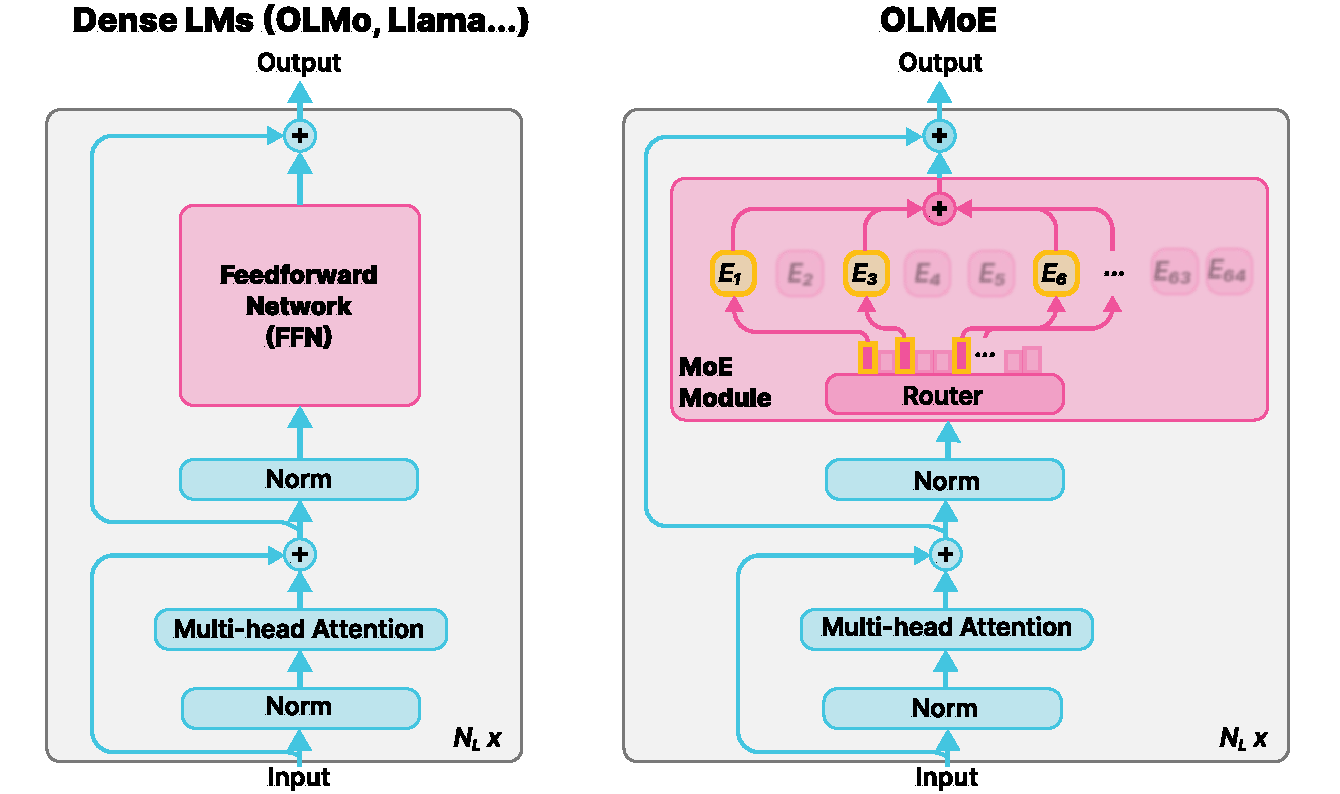
\includegraphics[width=0.9\linewidth]{figures/olmoe.pdf}
    \caption{混合专家模型（以OLMoE\cite{Muennighoff2024OLMoEOM}为例）和稠密模型的区别}
    \label{fig:densevsmoe}
\end{figure}

\paragraph{条件计算}

条件计算（Conditional Computation）是现代混合专家模型的核心思想。传统的神经网络在处理所有输入时，都使用完全相同的参数集合。与之相反，混合专家模型包含多个“专家”子网络，并为每个输入动态地选择一小部分专家来处理。这意味着，尽管模型的总参数量可以非常庞大（例如，由成百上千个专家组成），但对于单个输入词元（token）的处理，其计算路径是稀疏的，实际参与计算的参数量和计算量都远小于总参数量。这种方式打破了模型总参数量与计算量之间的固定耦合关系，使得在有限的计算预算下构建参数规模极其庞大的模型成为可能 \cite{Shazeer2017OutrageouslyLN}。

\paragraph{专家}
专家（Experts）是混合专家模型中执行具体计算的子网络。在基于Transformer的语言模型中，专家通常就是前馈网络（FFN）。假设一个MoE层有 $N$ 个专家，对于输入向量 $x$，第 $i$ 个专家 $E_i$ 的计算过程与其替代的密集FFN层一致：
\begin{equation}
E_i(x) = \text{GELU}(xW_{1,i} + b_{1,i}) W_{2,i} + b_{2,i}
\end{equation}
每个专家 $E_i$ 都拥有自己独立的参数 $\{W_{1,i}, b_{1,i}, W_{2,i}, b_{2,i}\}$。在训练过程中，通常认为，不同的专家会趋向学习并“专精于”处理不同类型的数据模式\cite{Xue2024OpenMoEAE}。

\paragraph{路由器 (Router)}
路由器的作用是为每个输入的词元 $x$ 决定应该由哪些专家来处理。它通过一个可学习的线性变换 $W_g$ 计算每个专家的得分（logits）：
\begin{equation}
h(x) = x W_g
\end{equation}
其中 $h(x) \in \mathbb{R}^{N}$ 是一个包含 $N$ 个专家得分的向量。在稀疏的Top-k路由策略中，路由器会从 $h(x)$ 中选择得分最高的 $k$ 个值。设这 $k$ 个专家的索引集合为 $\mathcal{T}$。然后，仅对这 $k$ 个得分应用Softmax函数（或其他激活函数）来计算它们的权重（门控值）：
\begin{equation}
G(x)_i = \begin{cases} \frac{e^{h(x)_i}}{\sum_{j \in \mathcal{T}} e^{h(x)_j}} & \text{if } i \in \mathcal{T} \\ 0 & \text{if } i \notin \mathcal{T} \end{cases}
\end{equation}
最终，混合专家模型层的输出 $y$ 是被选中的 $k$ 个专家输出的加权和：
\begin{equation}
y = \sum_{i \in \mathcal{T}} G(x)_i \cdot E_i(x)
\end{equation}
这个公式清晰地体现了条件计算的本质：只有索引在 $\mathcal{T}$ 中的少数专家被激活并参与计算，而它们的贡献由路由器动态计算的权重 $G(x)_i$ 决定。

\paragraph{专家并行}
专家并行（Expert Parallelism）（图\ref{fig:ep}）是专门为混合专家模型设计的一种模型并行（Model Parallelism）策略，旨在解决其巨大的内存占用问题。在标准的数据并行中，每个计算设备（如GPU）都保存一份完整的模型副本，这对于拥有数万亿参数的混合专家模型来说是不可行的。专家并行策略则将混合专家模型层中的 $N$ 个专家划分到 $M$ 个设备上，每个设备仅负责存储和计算其中的 $N/M$ 个专家。模型中的共享部分（如自注意力层和路由器）则在所有设备上进行复制。在训练的前向传播过程中，每个设备上的路由器为本地的词元批次做出路由决策。随后，通过一个高效的All-to-All通信操作，将需要由特定专家处理的词元发送到持有该专家的相应设备上。在各自的设备上完成专家计算后，再通过另一次All-to-All通信将计算结果发送回原始设备进行加权求和。这种方式虽然引入了额外的通信开销，但它极大地降低了单个设备的内存需求，使得训练远超单卡内存容量的巨型混合专家模型成为可能。

\begin{figure}[h]
    \centering
    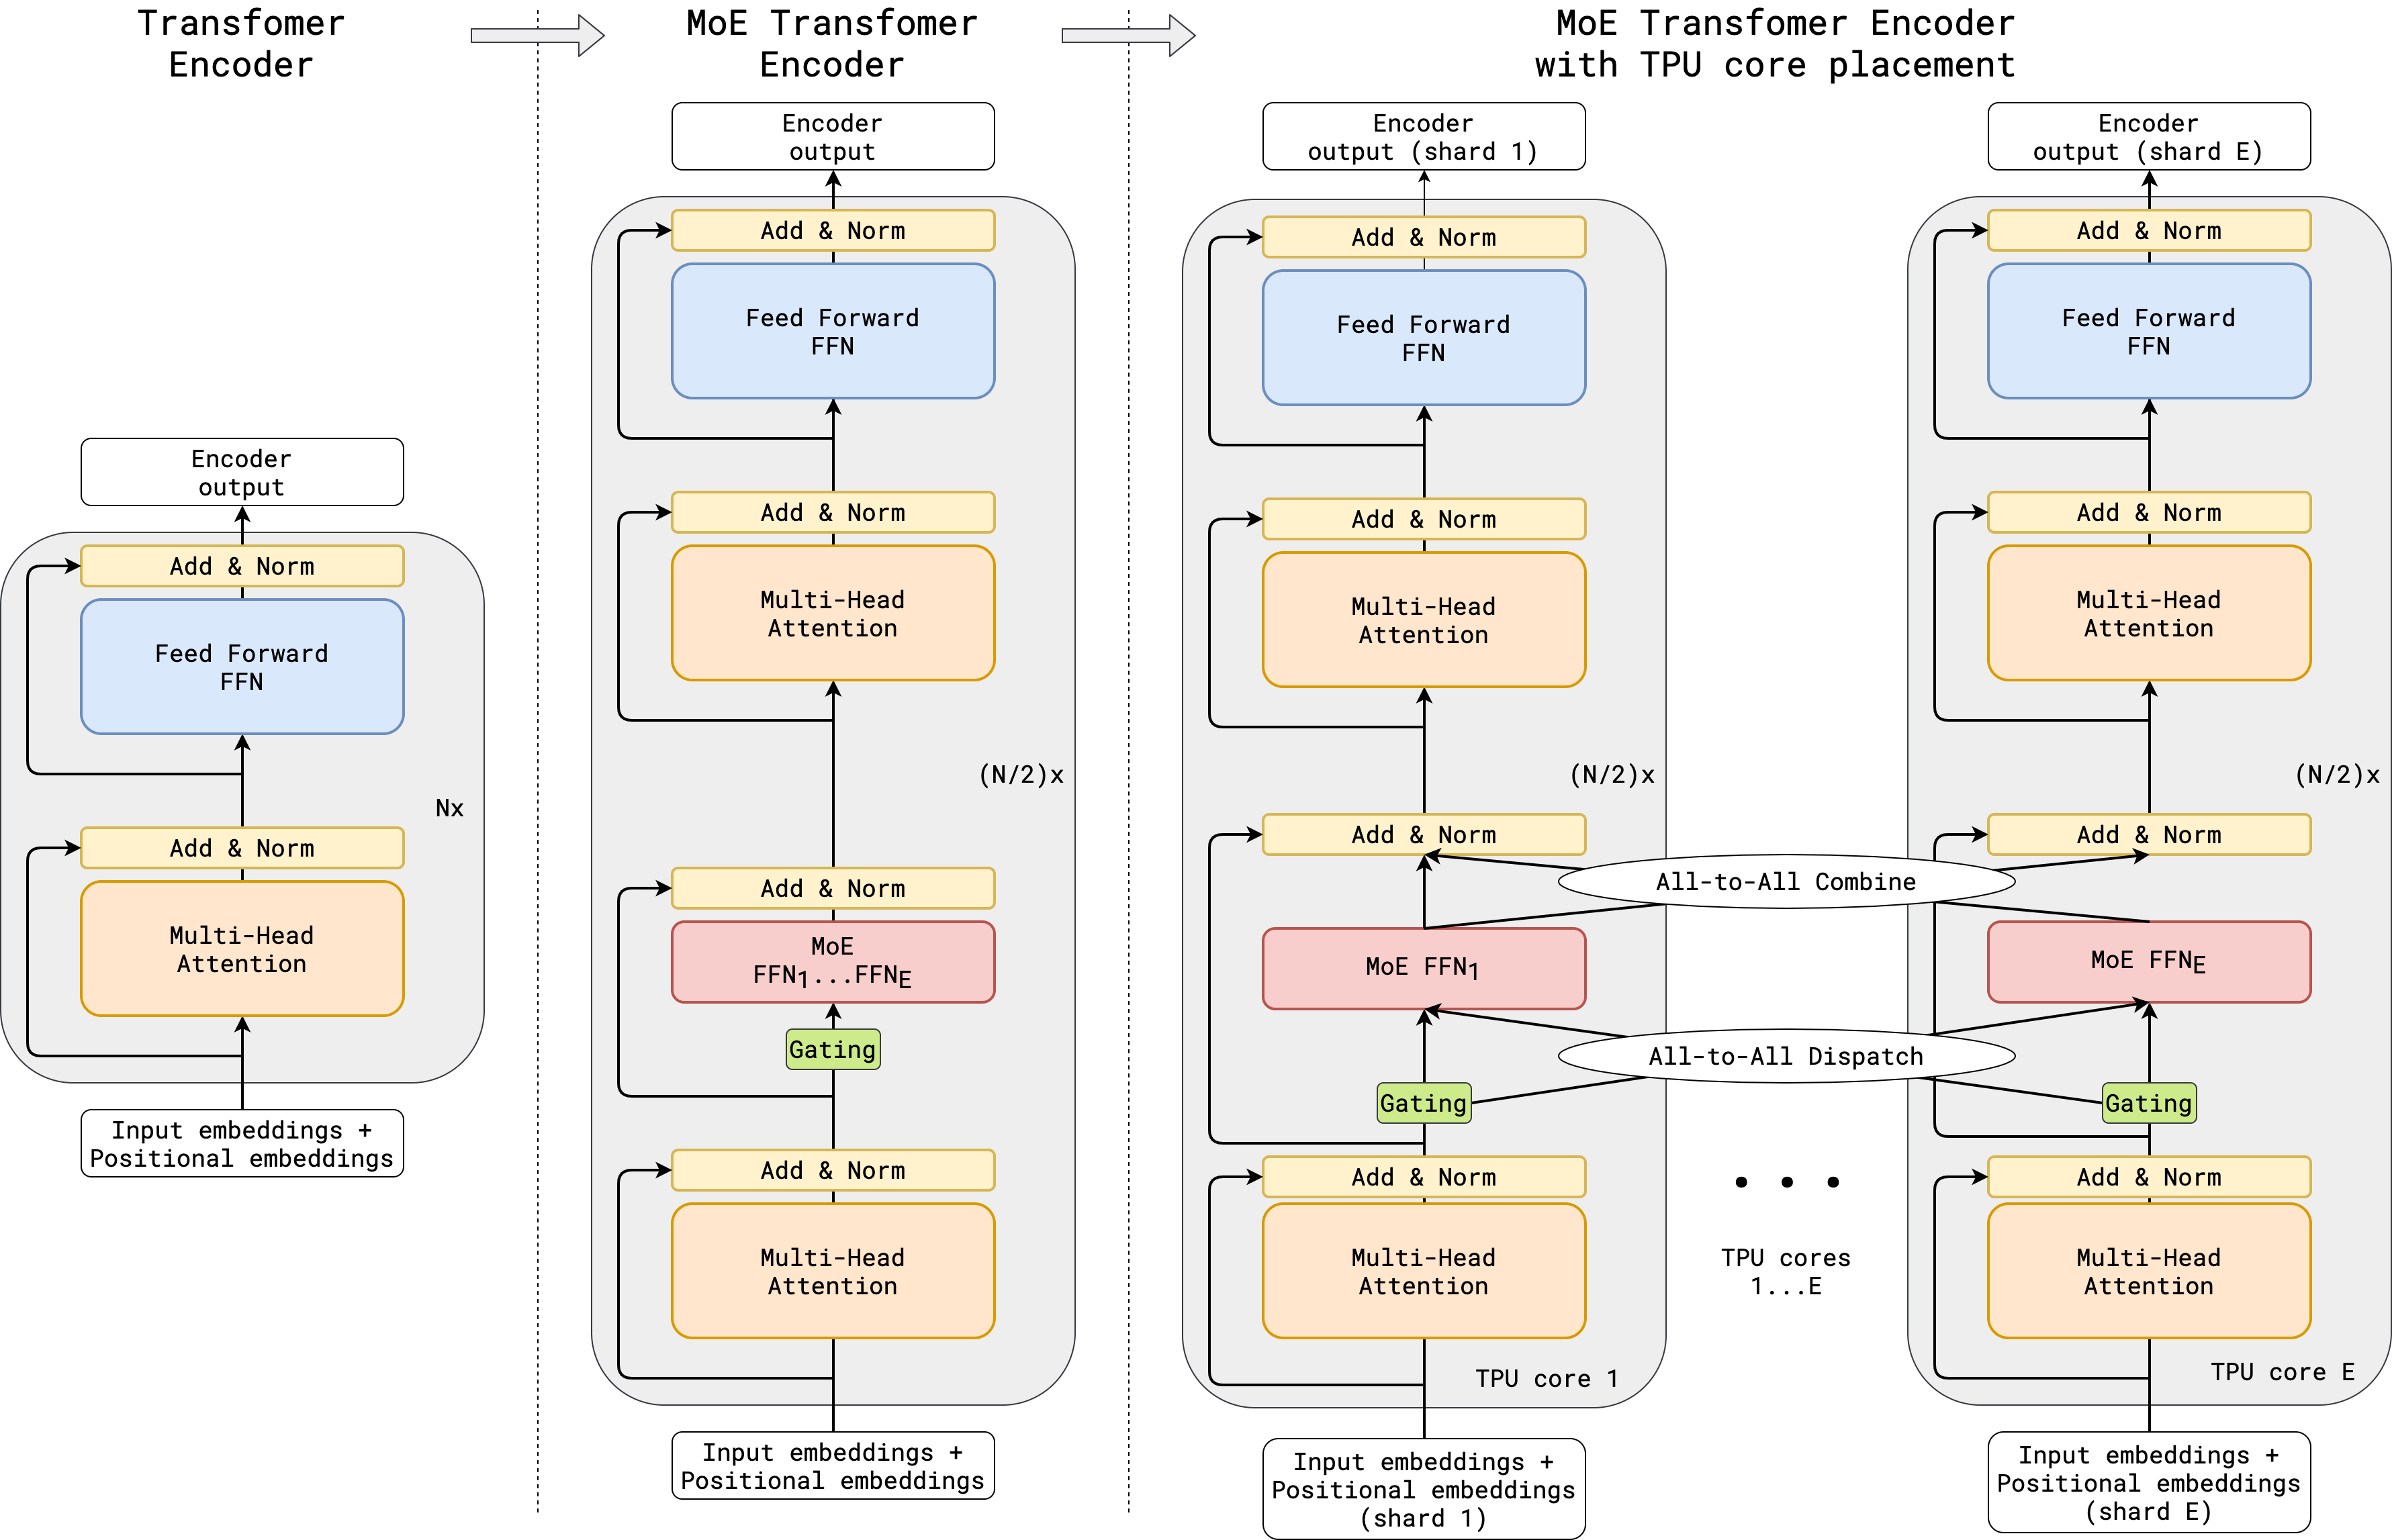
\includegraphics[width=1.0\linewidth]{figures/moe.png}
    \caption{GShard\cite{Lepikhin2020GShardSG}中的专家并行（以编码器部分为例，解码器亦类似）}
    \label{fig:ep}
\end{figure}

\section{预训练大语言模型}

预训练大语言模型（Pre-trained Large Language Models, LLMs）是指在一系列大规模、多样化的无标注文本语料上进行预训练，然后在各种下游任务上进行微调（fine-tuning）或在零/少样本（zero/few-shot）场景下使用的模型。这一范式已成为现代自然语言处理的基石，其成功的核心在于通过大规模数据和模型参数，让模型学习到通用的语言表征和世界知识。

\paragraph{自监督预训练}
LLMs 的核心技术是自监督学习（Self-supervised Learning）。与需要大量人工标注数据的监督学习不同，自监督学习从无标注数据本身创造学习信号。在NLP领域，主要有两种主流的预训练目标：
\begin{itemize}
    \item \textbf{自回归语言建模 (Autoregressive Language Modeling)}: 这是GPT系列模型 \cite{Radford2018ImprovingLU} 采用的核心目标。模型被训练来预测序列中的下一个词元（token），其目标函数是最大化给定上文条件下，下一个真实词的条件概率。对于一个词元序列 $X = (x_1, x_2, \dots, x_T)$，其似然函数为：
    \begin{equation}
    L(X) = \sum_{t=1}^{T} \log P(x_t | x_{<t}; \Theta)
    \end{equation}
    其中 $\Theta$ 代表模型参数。这种从左到右的单向建模方式天然适用于文本生成任务。

    \item \textbf{掩码语言建模 (Masked Language Modeling, MLM)}: 这是BERT \cite{Devlin2019BERTPO} 及其变体所开创的目标。训练时，输入序列中会随机遮盖（mask）掉一部分词元，模型的任务是根据其左右双向的上下文来预测这些被遮盖的词元。这种方式使得模型能够学习到深度的双向语境表征，因此在自然语言理解（NLU）任务上表现尤为出色。
\end{itemize}
通过在数千亿甚至上万亿词元的语料上进行预训练，模型能够内化丰富的语法结构、语义关系、语用知识乃至海量的世界知识。

\paragraph{从微调到上下文学习的范式演进}
早期的预训练模型（如BERT）主要遵循“预训练-微调”范式。模型首先完成通用知识的学习，然后针对特定的下游任务（如情感分析、命名实体识别等），使用该任务的标注数据对模型的全部或部分参数进行微调。然而，随着模型规模的急剧增大（如GPT-3达到1750亿参数），一种新的、更灵活的交互范式——\textbf{上下文学习}（In-Context Learning, ICL）——应运而生\cite{Brown2020LanguageMA}。上下文学习指的是大语言模型能够在不更新任何模型权重的情况下，仅通过在输入提示（prompt）中提供任务描述和/或少数示例，就能理解并执行新任务。这种能力根据示例的数量分为：
\begin{itemize}
    \item \textbf{零样本学习 (Zero-shot Learning)}: 只提供任务的自然语言描述，不提供任何示例。
    \item \textbf{少样本学习 (Few-shot Learning)}: 提供任务描述和少量（通常为1到几十个）输入-输出示例。
\end{itemize}
上下文学习的出现极大地降低了模型适应新任务的门槛，使得与单一模型进行对话式交互来解决多种问题成为可能，这也是当前大语言模型应用的主流形式。

\paragraph{缩放法则}
研究表明，大语言模型的性能与其规模之间存在着紧密且可预测的关系，这被称为\textbf{缩放法则} (Scaling Laws)\cite{Kaplan2020ScalingLF}。该法则指出，模型的性能（通常以测试集上的损失函数值来衡量）是模型所用计算量（C）、训练数据量（D）和参数量（N）的幂律函数（如图\ref{fig:scaling_law}所示）。这意味着，只要协同地、按比例地增加这三个要素，模型的性能就会持续提升。缩放法则为投入巨量资源构建更大模型提供了理论指导，也正是驱动模型走向万亿参数规模的根本动力。

\begin{figure}[h]
    \centering
    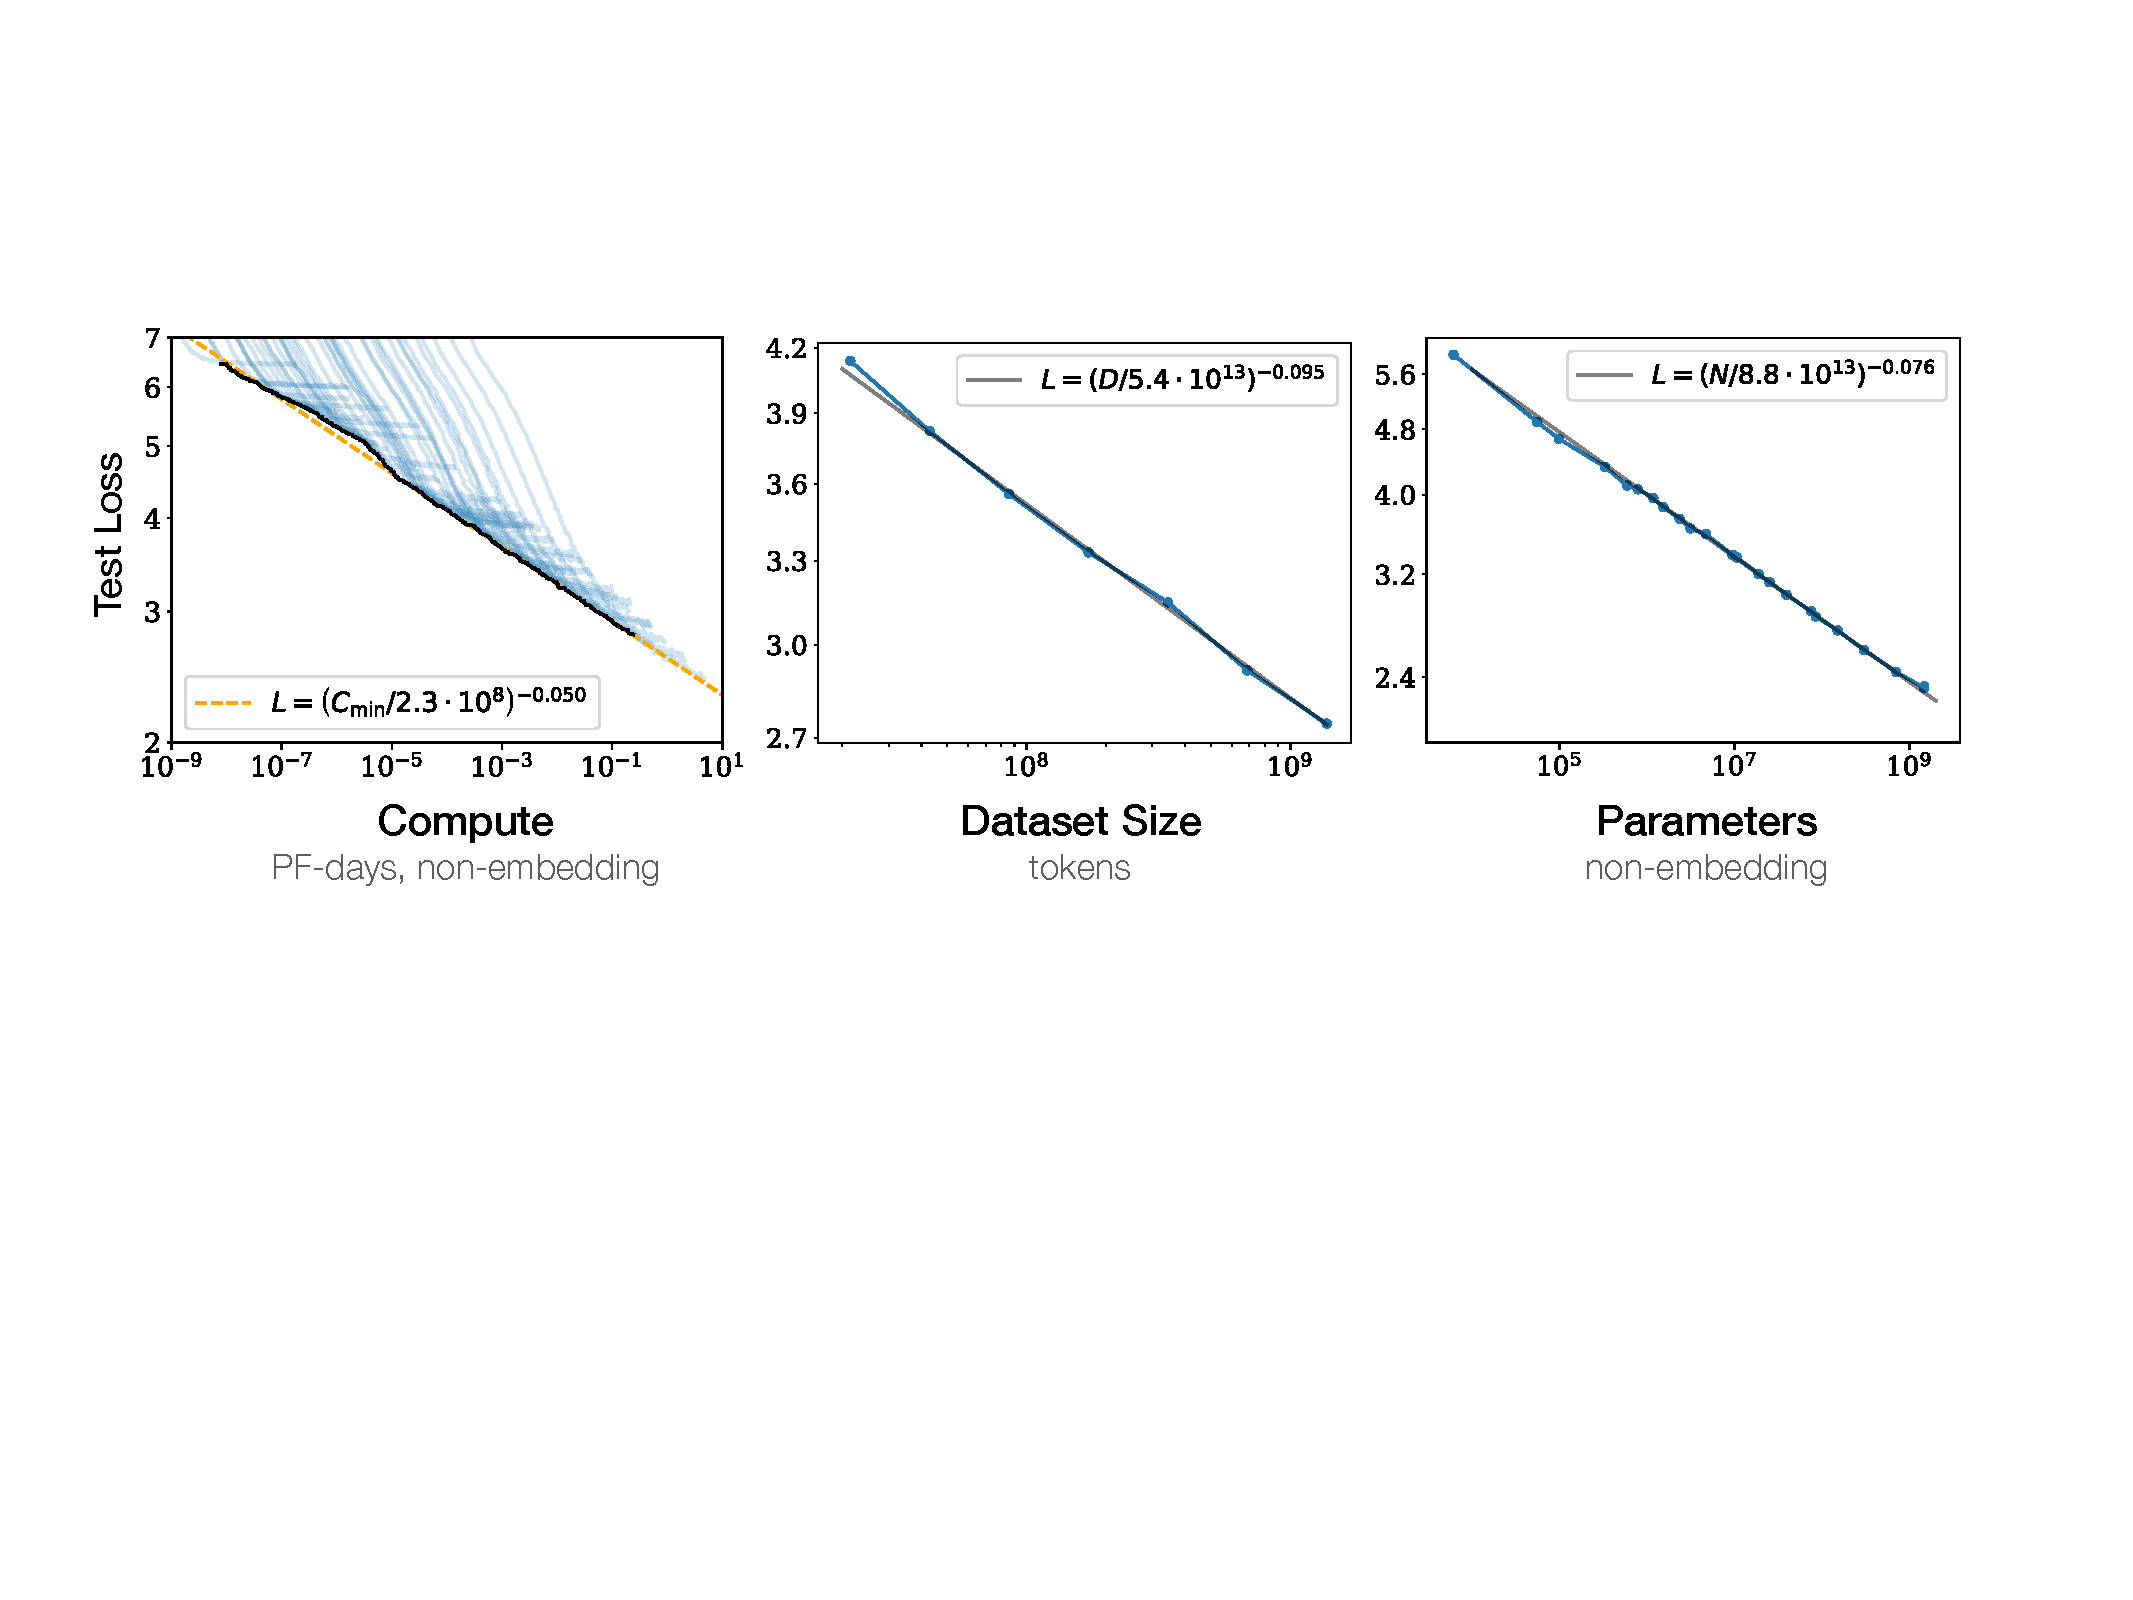
\includegraphics[width=1.0\linewidth]{figures/SimplePowerLaws.pdf}
    \caption{缩放法则指出，模型的性能（测试集上的损失函数值）是模型所用计算量、训练数据量和参数量的幂律函数\cite{Kaplan2020ScalingLF}。}
    \label{fig:scaling_law}
\end{figure}


\paragraph{涌现能力} 有趣的是，当模型规模跨越某个临界点后，它们会表现出许多在小规模模型上未曾出现的\textbf{涌现能力} (Emergent Abilities) \cite{Wei2022EmergentAO}（图\ref{fig:emergent}）。这些能力并非随着模型规模的增大而平滑地提升，而是在某个规模上“突然”出现。典型的例子包括多步算术推理、遵循复杂指令的能力，以及“思维链”（Chain-of-Thought, CoT）推理能力\cite{Wei2022ChainOT}——即通过引导模型分步思考来解决复杂问题。这些高级认知能力的涌现，进一步印证了扩大模型规模与计算量的重要性。
\begin{figure}[h]
    \centering
    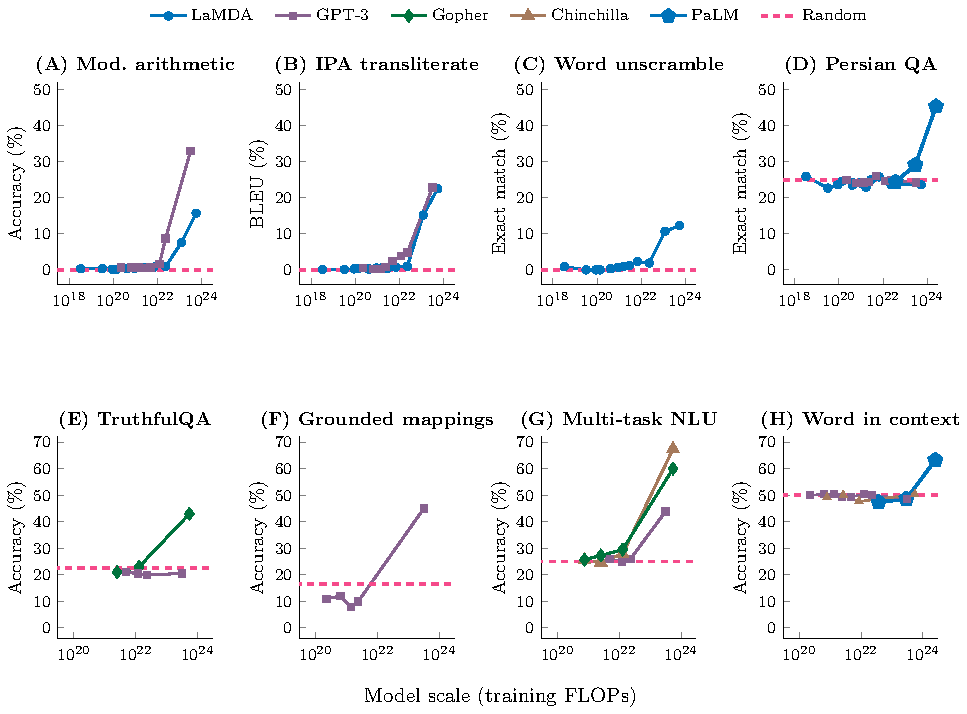
\includegraphics[width=1.0\linewidth]{figures/emergent.pdf}
    \caption{模型规模在跨越某个临界点后，展现出能力的突然提升\cite{Wei2022EmergentAO}。}
    \label{fig:emergent}
\end{figure}

\paragraph{训练效率与模型FLOPS利用率 (MFU)}
在实践中，要有效地实现缩放法则所预测的性能增益，仅仅提供理论上的计算量（FLOPs）是不够的，还必须确保硬件的计算潜力被充分利用。为此，业界提出了\textbf{模型FLOPS利用率}（Model FLOPs Utilization, MFU）这一关键工程指标 \cite{Chowdhery2022PaLMSL}。模型FLOPS利用率衡量的是在模型训练过程中，硬件（如GPU）实际达到的持续浮点运算速度与硬件理论峰值浮点运算速度的比率。一个高的模型FLOPS利用率意味着训练代码和系统架构能够高效地让硬件执行其最擅长的矩阵运算。然而，由于数据加载、GPU间的通信开销、非矩阵运算操作以及内存带宽限制等瓶颈，实现高模型FLOPS利用率是一项巨大的系统工程挑战。因此，优化训练效率、最大化模型FLOPS利用率，是降低训练成本、加速模型迭代、并最终在给定计算预算内触及缩放法则性能上限的核心环节。表\ref{table:training-efficiency}列出了一些模型的模型FLOPS利用率（MFU）。

\begin{table}[h!]
    \setlength{\tabcolsep}{6pt}
    \centering
    \small
    \begin{tabular}{lc cc}
    \toprule
     模型 & \makecell[c]{参数量(十亿)}  &  加速器芯片 & \makecell[c]{模型FLOPS利用率} \\
    \midrule
    GPT-3 & 175B &  V100 & 21.3\%  \\
    Gopher & 280B &  4096 TPU v3 & 32.5\%  \\
    Megatron-Turing NLG & 530B & 2240 A100 & 30.2\%  \\
    PaLM & 540B &  6144 TPU v4 & 46.2\% \\
    \bottomrule
    \end{tabular}
    \caption{一些模型的模型FLOPS利用率（MFU）\cite{Chowdhery2022PaLMSL}}
    \label{table:training-efficiency}
\end{table}

\paragraph{训练稳定性与损失尖峰的挑战}
在数百亿乃至万亿参数的规模下，预训练不仅是一项科学探索，更是一项对工程能力的巨大考验，其中\textbf{训练的稳定性}至关重要。在大规模训练中最常见也最棘手的失败模式是\textbf{损失尖峰 (loss spike)}：即训练损失（loss）突然发生灾难性的飙升，其值可能发散至无穷大 (`Inf`) 或变为无效数字 (`NaN`)。单次此类事件就足以破坏模型已学习到的权重，迫使研究人员中断进程，并回退到很早之前的稳定检查点 (checkpoint)，从而浪费数周甚至数月的宝贵计算资源。因此，理解并缓解这一不稳定性的根源，是LLM工程中的核心关切。

损失尖峰的根本原因是数值不稳定性，其来源多种多样：
\begin{itemize}
    \item \textbf{梯度爆炸 (Gradient Explosion)}\cite{Pascanu2012OnTD}: 这是最直接的原因。由于Transformer架构深度堆叠的链式特性，反向传播有时会导致梯度呈指数级增长。这会产生极大的权重更新，使得模型参数“越过”损失地貌 (loss landscape) 中的最优点，被抛入一个损失值高得多的区域，并可能再也无法从中恢复。

    \item \textbf{浮点数精度问题}: 为了加速训练并减少显存占用，LLMs通常采用低精度数值格式，其有限的动态范围使其极易出现上溢 (overflow，数值过大无法表示) 和下溢 (underflow，数值过小变为零) 的问题。为此，往往需要对不同模块设置合适的数值精度，并采取适当的量化方法，来保证训练的稳定性。

    \item \textbf{异常数据}: 庞大且通常混杂的预训练语料库中，可能包含格式错误或异常的数据点。这些数据点会产生异常大的损失值和梯度，从而成为触发不稳定的导火索。
\end{itemize}

为了应对这些问题，研究者们需要协同采用若干技术，如梯度裁剪（gradient clipping），权重衰减（weight decay）和归一化（Normalization）来稳定训练\cite{Rybakov2024MethodsOI,Wortsman2023SmallscalePF}。
在混合专家 (MoE) 模型中，这些挑战可能会变得更加复杂，因为其路由机制引入了额外的动态且可能不稳定的行为层（例如路由器的表示坍缩）。

% 这里补一张涌现能力的图片，然后后面再补一个概念/或者在moe那里补一个/或者前面补张图/最后补一下MFU的概念介绍？

% 后面moe可以提一下并行策略之类的，还有负载均衡;后面介绍的工作也可以讲讲偏向mlsys的？如果方便的话，写起来麻烦就算了
% 后面可以加一章介绍现代开源moe模型的典型结构
